\documentclass[a4paper,10pt]{article}

\usepackage{ifpdf}
\ifpdf
  \usepackage[pdftex]{graphicx}
  \graphicspath{{images/}}
\else
  \RequirePackage[dvipdfm, CJKbookmarks, bookmarks=true, bookmarksnumbered=true%
                unicode,%
             colorlinks,%
         citecolor=blue,%
             hyperindex,%
       plainpages=false,%
      pdfstartview=FitH]{hyperref}
  \AtBeginDvi{\special{pdf:tounicode UTF8-UCS2}}
  \usepackage[dvipdfm]{graphicx}
  \graphicspath{{images/}}
  \DeclareGraphicsExtensions{.eps}
\fi

%\RequirePackage{CJKutf8,CJKnumb,CJKulem}
\RequirePackage{CJKutf8,CJKnumb}
\RequirePackage{color,verbatim,cite}
\RequirePackage{texnames,makeidx,indentfirst}
\RequirePackage{amsmath,amssymb,amsfonts,bm,manfnt}
\RequirePackage{fancyhdr,titlesec,datetime}
\RequirePackage{wasysym,longtable,multirow,bigstrut}
\usepackage[section]{placeins}
\usepackage[left=3.2cm,right=2.54cm,top=3.3cm,bottom=2.6cm]{geometry}
\usepackage[caption=false,font=footnotesize]{subfig}

\AtBeginDocument{\begin{CJK*}{UTF8}{song}\CJKtilde\CJKindent\CJKcaption{utf8}}
\AtEndDocument{\end{CJK*}}

\setlength{\parskip}{0.75ex plus .2ex minus .5ex}
\renewcommand{\baselinestretch}{1.2}

\hypersetup {
    pdftitle={无线传感器网络中的位置相关安全研究},
    pdfauthor={杨文博}
}

\title{无线传感器网络中的位置相关安全研究}
\author{杨文博}

\begin{document}

\maketitle

\section{ 选题依据 } 

\subsection{课题的研究意义和国内外研究的概况}

\subsubsection{无线传感器网络及其中的安全问题}  

无线传感器网络(Wireless Sensor Network, WSN)在最近几年获得了全球的广泛关注。伴随着与传感器相关的通信、嵌入式和分布式计算技术的飞速发展,特别是微机电系统(Micro-Electro-Mechanical, MEMS)的长足进步,人们研制出了各种不同共用的廉价微型传感器。这些传感器可以感知、测量并收集所处的环境信息,并将这些信息通过某种方式传输给布置~WSN~的用户。它们可以被广泛应用于国防军事、国家安全、环境监测、火灾预警、交通管理、医疗卫生和灾难救援等许多领域,帮助人们获得大量有价值的目标环境信息。

无线传感器节点一般情况下由感应模块、处理器、内存、能量供应、无线模块和控制单元组成。装配着不同的感应模块的传感器可以感应物理环境的不同信息,例如湿度、温度、压力、震动、风速、声音、辐射、有毒气体含量等等。由于其廉价性和微型化,无线传感器所采用的处理器一般比较低端,不支持如浮点运算、多媒体指令等一些高级功能。无线传感器节点一般都只有少量的内存,它所收集到的信息将使用无线方式传输到基站。一般情况下,无线传感器节点的能源主要由电池供应,后备能源可以根据环境的不同采用太阳能等其它的能量供应方式。

无线传感器网络则是由大量无线传感器节点构成的分布式、自组织的无线网络。典型的无线传感器网络一般由数十到数千个无线传感器节点组成,用来检测一定范围区域内的环境信息。受无线传感器节点体积小、数量大、资源受限的限制,~WSN~往往具有以下特点:

\begin{enumerate}

\item 树形路由、多跳转发。WSN~需要将收集到的信息传回基站,所以一般构成以基站为根节点的树形结构;由于信号的覆盖范围受限,无线传感器节点间通信往往需要经过多跳转发,其转发由传感器节点完成,没有专门的路由设备。

\item 无线传输的带宽、稳定性和安全性较差。由于底层采用无线通信,受到信道本身物理特性的限制,~WSN~的通信质量和稳定性往往较差;考虑到无线信号的开放性,其更容易受到信道窃听、伪装、拒绝服务等攻击,需要特别考虑一些安全需求。

\item 网络资源受限。~WSN~中,无线节点往往不具有长期的电源供应,节点设计的计算能力、存储空间都要比一般的有线网络节点要小得多。在设计网络网络结构时需要特别考虑到能耗因素,避免部分节点能源耗尽导致整个网络失灵。

\end{enumerate}

\begin{figure}[htbp]
  \centering
  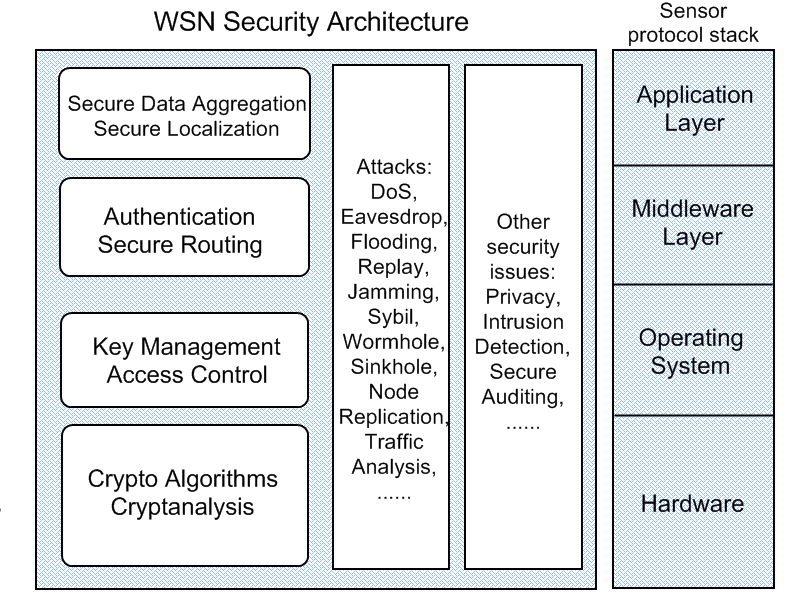
\includegraphics[width=0.8\textwidth,keepaspectratio]{wsn_sec_map}
  \caption{\label{wsn_sec_map}~WSN~安全架构~\cite{Li2005}}
\end{figure}

由于受以上条件限制,很多传统的安全措施难以使用在~WSN~上,而且~WSN~往往用于监测敏感信息或者部署在充满敌意的环境中,所以~WSN~在应用中面临着许多不同的安全问题和安全需求,如图~\ref{wsn_sec_map}~所示。

\begin{enumerate}

\item 数据安全。在~WSN~中,数据安全包括数据的保密性、完整性、新鲜性和数据源认证。数据的保密性要求节点获得的信息不泄露给其它节点、敏感信息传输安全以及抵抗流量分析;数据的完整性要求在传输的过程中数据不被敌手篡改;数据的新鲜性要求保证收到的数据是最新的而不是敌手重放的;数据源认证则使消息的接收者能够验证数据来源于其声称的发送者。数据安全一般通过密码学手段来达到~\cite{Perrig2002},同时这些密码学方法也是保证其它安全需求的基础。

\item 密钥管理和访问控制。由于计算和能量要求的限制,经典的密钥交换算法或公钥算法无法使用在~WSN~中,那么就造成密钥分配的困难。有效和安全的密钥管理,是达到网络可用性、鲁棒性和自组织的重要因素~\cite{Lee2007};传感器节点能量受限,合理地采用睡眠、侦听等访问控制方法能够有效地延长~WSN~的运行寿命。安全的时钟同步在访问控制中也起着非常重要的作用。

\item 路由安全。~WSN~一般组成树形结构,数据的传输通过多跳转发,如何避免敌手对路由协议的攻击,保证路由的安全、正确,是影响网络可用性的重要因素。

\item 安全定位。无线传感器在收集数据时,往往需要具体的位置信息,如果节点出了故障,也需要位置信息来定位故障,安全定位机制讨论在节点定位过程中检测和抵御攻击的方法。

\item 安全数据融合。在收集传感器数据的过程中,采用数据在网内融合后再上传,能够节省能量开销、增强信息的准确性和提高收集效率,安全数据融合讨论在融合过程中遇到的安全问题。

\end{enumerate}

\subsubsection{~WSN~中位置相关安全问题}  

在~WSN~监控的应用中,监控程序获得网络所收集到的环境信息,检测是否有事件发生。在一些事件发生时,传感器网络往往需要知道该事件发生的位置以及感知该事件的传感器节点的位置。因此,位置信息是~WSN~中的一项重要信息,有着非常广泛的应用,包括数据的识别和关联、节点定位、对指定区域节点的管理和查询、评估节点密度和覆盖范围、网络能量分布图、基于地理位置的路由、目标追踪和其它位置应用~\cite{Boukerche2007a,Yick2008}。

这里我们主要讨论位置信息的安全获得及其应用方面遇到的安全问题,对~WSN~位置信息的攻击主要有以下几种类型:

\begin{itemize}

\item 对距离/角度估计方法的攻击(Attacks on distance/angle estimation)~\cite{Boukerche2008}。在目前的定位机制中,传感器节点通常使用信号强度、到达时间或者跳数估计等方法测量节点间距离,或者用定向天线、接收阵列等方法来估计节点间角度~\cite{Boukerche2007a}。在对距离估计的方法进行攻击时,敌手可以利用攻击节点用更高或者更低的强度发送信号、故意延迟数据包的发送时间或者传播错误的跳数来使邻居节点产生错误的距离判断;也可以采用改变物理介质的方法,比如添加信号噪音、障碍物和烟雾,来改变物理信道的性质以使距离判断产生较大误差。在对角度估计方法进行攻击时,敌手也可以在环境中布置磁铁来改变物理信道的性质。

\item 对位置计算的攻击(Attacks on position computation)~\cite{Boukerche2008}。当一个传感器节点获得了足够的邻居节点的位置信息之后,就可以用三角计算、三边计算、多边计算、极大似然估计、质心算法等方法来计算自身的位置~\cite{Boukerche2007a}。目前来讲对位置计算的攻击主要表现为传播虚假的位置信息,或者无线信号干扰,比如干扰~GPS~信号使参考节点无法获得自身的位置,也使得以其为参考的~WSN~节点无法正常计算位置。

\item 对定位算法的攻击(Attacks on the localiation algorithm)~\cite{Boukerche2008}。定位算法是~WSN~定位系统的主要组成部分。定位算法决定了如何传播和利用位置信息来使得整个网络中的节点都可以计算到自身的位置~\cite{Boukerche2007a}。由于~WSN~的分布式特性,~WSN~中的定位算法也拥有其它分布式系统的弱点。典型的攻击方式有女巫攻击(Sybil Attack)、重放攻击(Replay Attack)和虫洞攻击(Wormhole Attack)。

\item 对位置信息私密性的攻击(Attacks on location privacy)~\cite{Gruteser2003}。敌手可以通过被动地侦听、流量分析,或者主动地插入错误数据、改变路由行为来获得定位系统的信息,进而得到目标节点的位置和其它私密信息。

\end{itemize}

由于~WSN~容易受到以上几种攻击,就需要研究安全的定位和路由算法来保证位置信息的正确、安全地获得和使用。同时,正确的~WSN~中节点的位置信息也会帮助发展更可靠的安全服务,比如基于位置信息的对偶或组密钥建立方法~\cite{Liu2003,Huang2004}。

\subsubsection{国内外研究现状}  

WSN~安全定位技术是一个比较新的研究课题,对其系统的研究起源于~2003~年左右。目前来讲,~WSN~的安全定位技术按照其算法可以大致分为用密码学手段、异常行为检测和屏蔽、容忍攻击的鲁棒位置算法和位置验证技术等几大类~\cite{Boukerche2008},如图~\ref{wsn_sec_pos}~所示。下面我们对这几大类技术进行一些简单的说明和分析。

\begin{figure}[htbp]
  \centering
  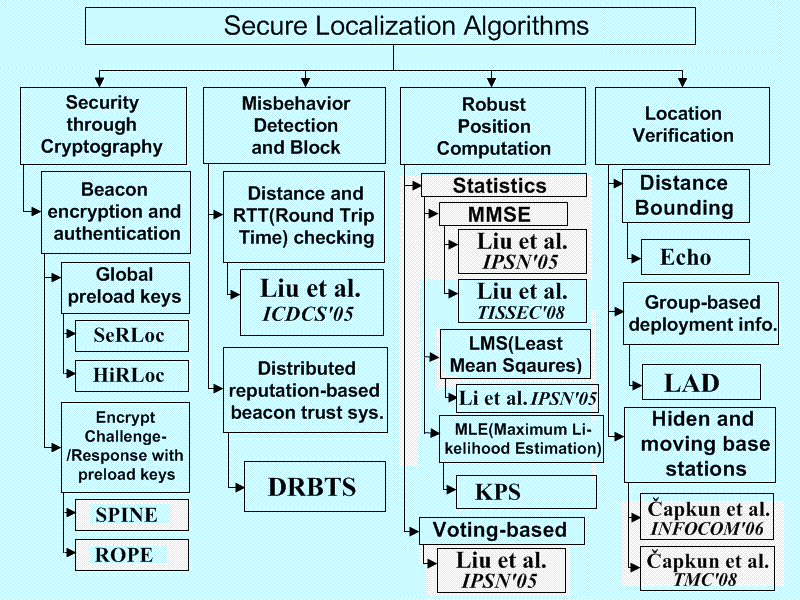
\includegraphics[width=.9\textwidth,keepaspectratio]{wsn_sec_pos}
  \caption{\label{wsn_sec_pos}~WSN~安全定位算法}
\end{figure}

\begin{itemize}

\item 密码学手段(Security through Cryptography)。密码学是保证信息安全的重要工具之一,因此也被广泛用于保护定位系统传输数据的安全中。数据包加密和数据源认证是安全定位系统中被广泛采用的密码学手段。

L. Lazos~和~R. Proovendran~等人提出的~SeRLoc \cite{Lazos2005}、~ROPE \cite{Lazos2006}~和~HiRLoc \cite{Lazos2005a},S. \v{C}apkun~和~J.P. Hubaux~提出的~SPINE \cite{Capkun2005, Capkun2006}~等方案,都采用了加密和数据源认证方法来保证~beacon~消息的安全传输。其中~SeRLoc~主要依靠已知自身位置的定位者节点,利用定向天线向扇形区域广播包含其自身位置和扇区信息的~beacon~信号,其它节点通过接收到的~beacon~信号判断自己处于哪些扇区内,这些扇区相交区域的重心就是该节点的位置。SeRLoc~采用全局的密钥来加密~beacon~消息,用私密口令的~hash~值链实现对~beacon~的消息源认证~\cite{Lazos2005}~(range-independent);SPINE~中提出了可验证的多向法(Verifiable Multilateration),第一次将距离边界协议(Distance Bounding Protocol)引入~WSN~位置验证中,在~VM~中至少三个验证节点独立使用距离边界协议计算某节点的位置,并将计算得的距离上传到一个~CA(Central Authority)~,CA~使用最小均方误差(Minimum Mean Square Error, MMSE)或者其它方法来估计得该节点的位置,并验证其是否在误差范围和扇区相交区域内,如果是就承认该距离估计有效。在~SPINE~方案中,距离边界协议使用了加密的挑战应答过程,需要节点与定位者共享对偶密钥~\cite{Capkun2005}~(range-based);ROPE~方案在~SeRLoc~基础上增加了距离边界协议,节点和能与其双向通信的定位者节点计算可信距离,配合扇区相交区域计算出节点位置。节点同样可以使用距离边界协议向某定位者节点证明自己在某位置附近,但是~ROPE~的过程不需要~CA~的参与。ROPE~同样要求所有节点与所有定位者共享对偶密钥~\cite{Lazos2006};HiLoc~是在~SeRLoc~的基础上,利用可旋转和可变发射功率的定向天线来达到高精度定位的目的。它与~SeRLoc~相同,也使用全局的密钥来加密~beacon~消息,用私密口令的~hash~值链实现对~beacon~的消息源认证~\cite{Lazos2005a}。

\item 异常行为检测和屏蔽(Misbehavior Detection and Block)。防范对定位系统的攻击还可以使用检测恶意节点的异常行为并屏蔽该恶意节点的方法。此方法主要用来防范对定位算法中位置计算部分的攻击。D. Liu~等在~\cite{Liu2005c}~提出了两个检测恶意~beacon~节点的方法:一个是节点用其与目标节点的坐标距离和实测距离(由信号估计得来)相比较,如果误差大于某个阈值,就认为该目标节点传输了虚假的坐标值,视其为恶意节点;另一个是节点用其与目标节点的通信往返时间与正常往返时间比较,如果误差大于某个阈值,则认为该目标节点进行了重放攻击,视其为恶意节点。A. Srinivasan~等在~\cite{Srinivasan2006}~中提出了一个分布式的基于信誉的~becon~信任系统(Distributed Reputation-based Beacon Trust System, DRBTS)。每个~beacon~节点维护一个邻居~beacon~节点的信誉表(Neighbor-Reputation-Table, NRT),节点间交换~NRT~,使用基于投票的方式选择可信节点组。

\item 容忍攻击的鲁棒位置算法(Robust Position Computation)。解决恶意节点问题的另一种办法是接受恶意节点存在这一现实,使用鲁棒的位置计算方法来消除恶意信息的影响。研究者一般假设正常节点多于恶意节点,然后使用统计或者异常值过滤(outlier filtering)技术来实现消除恶意节点影响的目标。这些方法一般用来防范对定位算法中位置计算或者位置/角度估计部分的攻击。

D. Liu~等在~\cite{Liu2005b}~中提出了攻击容忍的两个方案:第一个方案利用最小均方误差估计(Minimum Mean Square Estimation, MMSE)来识别并排除恶意节点。节点首先用基于~MMSE~的方案估计自身位置,然后看该位置能否由一个一致的参考者节点集合推出(距离估计的均方误差作为非一致性的参数),如果均方误差比较大,那么就剔除参考点集合中最不一致的节点重新估计位置,直到所有非一致节点都被剔除;第二个方案基于投票机制。WSN~部署区域被量化成网格,每个参考者节点对某节点所在位置进行投票,得票数最多的网格区域中央被选为该节点所在位置,这样能降低恶意节点在网络中的作用。D. Liu~等在~\cite{Liu2008a}~中又改进了~\cite{Liu2005b}~中提出的方案,提出一个增强的贪心~MMSE~算法(Enhanced Greedy Algorithm, EARMMSE),使用贪心算法减少了恶意节点识别和排除过程的计算量。

L. Fang, W. Du~和~P. Ning~在~\cite{Fang2005}~中提出了一个不需要~beacon~节点的位置计算方案~KPS(deployment Knowledge-based Positioning System),在~KPS~中节点根据预知的部署信息和当前的邻居节点,使用最大似然估计(Maximum Likelihood Estimation, MLE)方法计算自身可能的位置。该方案可以容易小部分邻居节点是恶意节点的情况。

Z. Li~等在~\cite{Li2005a}~中提出了使用自适应的最小二乘法(Least Squares, LS)和最小均方算法(Least Mean Squares, LMS)的统计方法来容忍对定位算法的攻击。具体做法是在使用三角方法(Triangulation)估计节点位置时,无攻击存在时使用~LS~算法,当有攻击存在时使用~LMS~算法,因为~LMS~算法能够容忍不超过~50\%~的异常值并且获得正确估计。

\item 位置验证技术(Location Verification)。位置验证也是安全定位研究中非常重要的一个方面,它将视角从直接解决安全定位问题转向验证定位结果是否正确。我们前文中提到的一些方案,比如~SPINE \cite{Lazos2005a}, ROPE \cite{Lazos2006}~和~HiLoc \cite{Lazos2005a}~,也在安全位置计算过程中加入了位置验证过程。

N. Sastry~等在~\cite{Sastry2003}~中首先提出安全位置验证(Secure Location Verification)的概念,并给出了一个~Echo~方案,主要原理是使用无线射频和超声波测距的距离边界协议。原始~Echo~方案中使用~nonce~来抵御重放攻击,~\cite{Sastry2003}~中也提到在存在共享密钥的情况下,可以使用共享密钥来对消息源进行认证。

W. Du, L. Fang~和~N. Peng~基于~KPS~\cite{Fang2005},提出了一个在定位过程结束后,检测位置异常的节点~LAD(Localization Anomaly Detection)~\cite{Du2006}~方案。此方案中,节点被分组部署,根据部署信息和定位结果,若某节点的声称位置与其所属组节点的位置差距过大,则认为该节点位置异常。

S. \v{C}apkun, M. \v{C}agalj~和~M. Srivastava~提出了利用可信的隐藏和移动基站来对节点的位置进行验证的方案~\cite{Capkun2006a, Capkun2008}。由于部分基站位置隐藏(无线电静默)或者移动,攻击者无法判断该类基站位置,该类基站通过监听信道可以获得更真实的数据,判断节点是否处于声称的位置。

\end{itemize}

目前保护~WSN~节点位置信息私密性的研究并不多。~M. Gruteser~等在~\cite{Gruteser2003}~中首先提出使用数据隐藏(降低数据精度)、分层数据融合和加密通信的方法保证位置信息的私密性;C. Ozturk, Y. Zhang~和~W. Trappe~提出了利用抵抗流量分析的手段来防止敌手通过追踪通信得到节点位置,主要使用随机路由和增加虚假流量的方式~\cite{Ozturk2004},这些方式的主要问题是为了达到匿名性引入不必要的通信,因而使得能量消耗过大~\cite{Xiao2006};Y. Xi~等对~C. Ozturk~的方法进行了改进,提出了使用双向贪心随机游走的~GROW(Greedy Random Walk)~方案~\cite{Xi2006},~GROW~要求消息的发送者和接收者都进行若干跳的随机游走,当发送者和接收者的随机游走路径发生交叉时,就用该路径进行消息的传输。

~WSN~节点的位置信息在其它安全服务中也有一定的应用。D. Liu~和~Peng Ning~认为可以利用~WSN~节点的部署信息来减少密钥预分配的复杂度,提出了两个方案:CPKS(Closest Pairwise Keys Scheme)~和~LBKP(Location-Based Key Predistribution)\cite{Liu2003}。前者利用准确的周围临近节点信息预分配对偶密钥,后者将部署区域划分成块,使用基于二元多项式的密钥预分配方法来为每块区域中的节点分配对偶密钥;D. Huang~等在~\cite{Huang2004}~中提出了将~SK-RKP (Structured Key-pool Random Key Predistribution)~算法应用到分组按网格部署的~WSN~网络上,每个节点存储密钥所需空间比不利用部署信息要少将近~3~倍。

\section{研究内容和研究方法} 

\subsection{研究内容}

\begin{enumerate}

\item 探索更适合~WSN~的简单的安全定位方法。目前的~WSN~安全定位方法一般要求~beacon~节点携带~GPS~定位仪,或者携带定向天线,或者需要更多的基站,所以在实际应用上依然有困难。我们希望能考虑到~WSN~的现状,提出一个安全保护级别和当前设备以及网络性能相适应的算法。

\item 寻找更稳健的安全定位算法。在异常节点的识别和排除方面,目前比较多的是使用统计和选举的手段,寻找更合适的方法,使定位算法所需计算量更小而不影响定位精度。

\item 设计通信开销与隐私保护强度更均衡的位置信息私密性保护方案。目前的位置信息私密性保护方案主要采用在网络中引入虚假流量来迷惑敌手,这样所带来的通信开销比较大,我们希望能找到一个更均衡的私密性保护方案。

\item 将安全定位算法与其它安全方案结合考虑。由于安全定位算法与其它的安全方案可以共享一些信息和模块,我们可以将它们结合一起考虑,也许会发现更优的算法。

\end{enumerate}

\subsection{研究方法}

\begin{enumerate}

\item 综合评估现有安全定位方法的特点与不足。

\item 对目前基于统计的鲁棒安全定位算法进行详细研究。

\item 将安全定位方案与其它安全方案比较,找出共同可利用的信息和模块。

\item 提出新的安全方案的细节。

\item 提出对安全定位和隐私保护通信开销估量的指标。

\item 对多个安全方案进行模拟和比较。

\end{enumerate}


\section{课题研究的创新之处}

未完成

\section{研究工作进度安排}

未完成

\section{已取得的与论文研究内容相关的成果} 

无。

\bibliographystyle{IEEEtran}
\bibliography{IEEEfull,wsn}

\end{document}

